
\section{Continuity}
\begin{frame}
    \frametitle{Definition of Continuity}
    A function $f$ is continuous at a number $a$ if
    \begin{center}
        $\lim\limits_{\textit{x} \to a} = f(a)$
    \end{center}
    This definition actually implicitly requires three things:
    \begin{enumerate}
        \item $f(a)$ is defined
        \item $\lim\limits_{\textit{x} \to a}f(x)$ exists
        \item $\lim\limits_{\textit{x} \to a}f(x) = f(a)$
    \end{enumerate}

    \frametitle{Definition of Continuity}
    A function $f$ is continuous from the right at a number $a$ if
    \begin{center}
        $\lim\limits_{\textit{x} \to a^{+}} = f(a)$
    \end{center}
    A function $f$ is continuous from the left at a number $a$ if
    \begin{center}
        $\lim\limits_{\textit{x} \to a^{-}} = f(a)$
    \end{center}
\end{frame}
\begin{frame}
    \frametitle{Definition of Continuity}
    A function is continuous on an interval if it is continuous at \alert{every number in the interval}. (If $f$ is defined only on one side of an endpoint of the interval, we understand \textit{continuous} at the endpoint to mean \textit{continuous from the right} or \textit{continuous from the left}.)
\end{frame}

\begin{frame}
    \frametitle{Theorem 1}
    If $f$ and $g$ are continuous at $a$ and $c$ is a constant, then the following functions are also continuous at $a$:
    \begin{enumerate}
        \item $f + g$
        \item $f - g$
        \item $cf$
        \item $fg$
        \item $\dfrac{f}{g}$\ \ \ \alert{(if $g(a) \neq 0$)}
    \end{enumerate}
\end{frame}
\begin{frame}
    \frametitle{Theorem 2}
    The following types of functions are continuous at every number in their domain(s):
    \begin{enumerate}
        \item polynomials
        \item rational functions
        \item root functions
        \item (inverse) trigonometric functions
        \item exponential functions
        \item logarithmic functions
    \end{enumerate}
\end{frame}
\begin{frame}
    \frametitle{Theorem 3}
    If $f$ is continuous at $b$ and $\lim\limits_{\textit{x} \to a}g(x) = b$, then $\lim\limits_{\textit{x} \to a}f(g(x))=f(b)$.\\
    \bigskip
    In other words,
    \begin{center}
        $\lim\limits_{\textit{x} \to a}f(g(x))=f(\lim\limits_{\textit{x} \to a}g(x))$
    \end{center}
\end{frame}
\begin{frame}
    \frametitle{Theorem 4}
    If $g$ is continuous at $a$ and $f$ is continuous at $g(a)$, then $f(g(x))$ is continuous at $a$.\\
    \bigskip
    \bigskip
    \textit{"A continuous function of a continuous function is a continuous function."}
\end{frame}
\begin{frame}
    \frametitle{Theorem 5-The Intermediate Value Theorem}
    Suppose that \alert{$f$ is continuous on the closed interval $[a,b]$} and let $N$ be any number between $f(a)$ and $f(b)$, where $f(a) \neq f(b)$. Then there exists a number $c$ in $(a,b)$ such that $f(c) = N$.\\
    Note that the value $N$ can be taken on once or more than once.
    \begin{figure}
        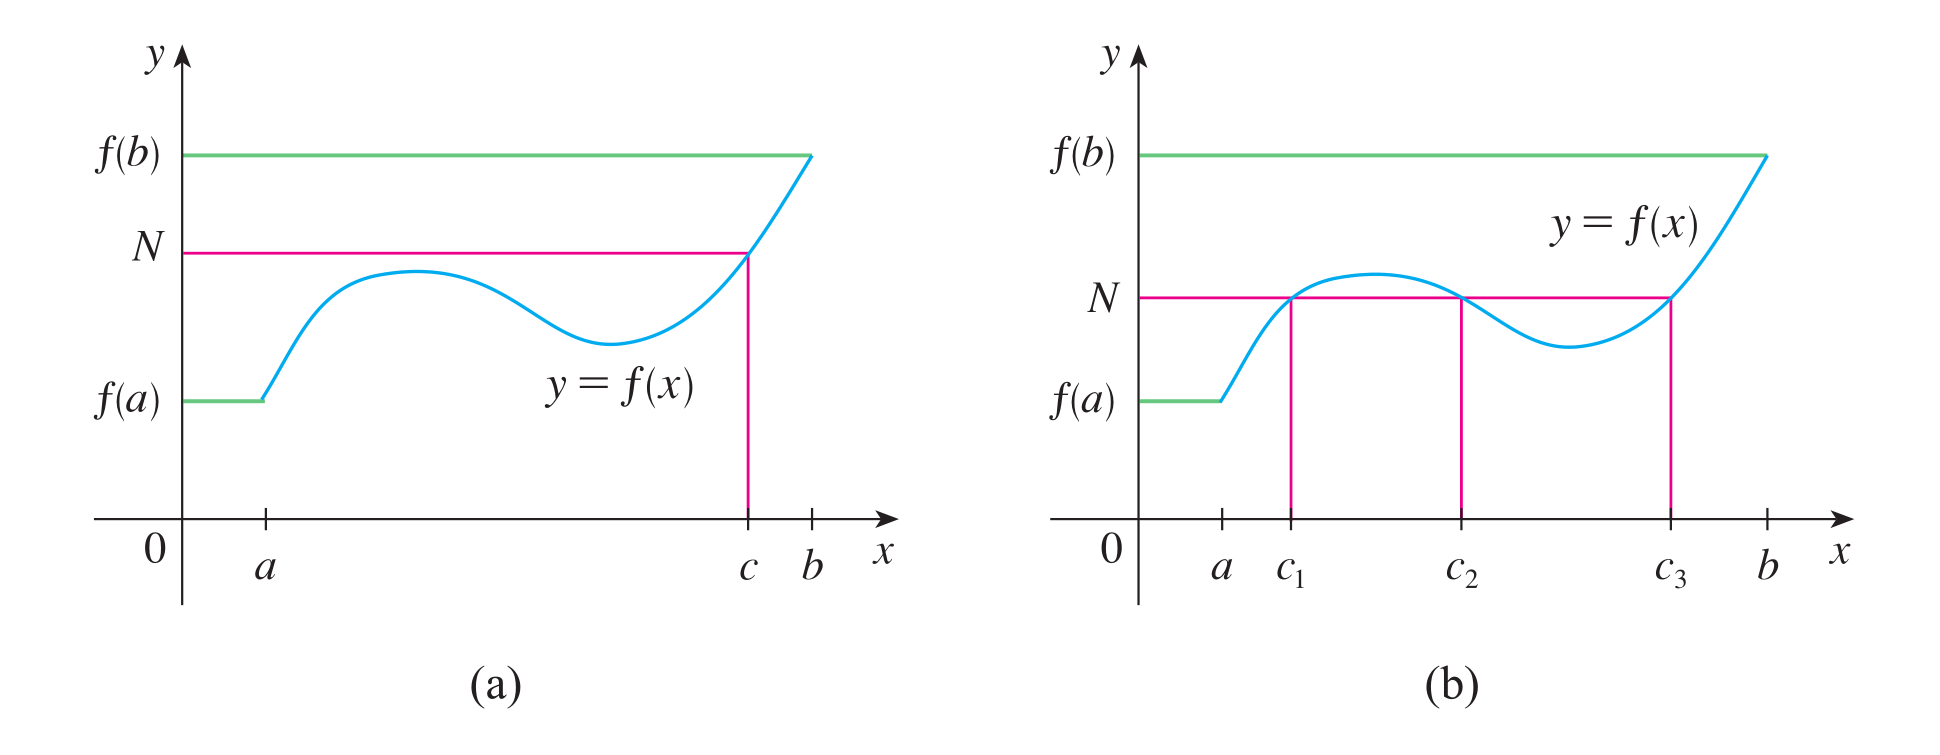
\includegraphics[width=0.9\linewidth]{res/in.png}
    \end{figure}
\end{frame}
\begin{frame}
    \frametitle{Types of Discontinuities}
    \begin{enumerate}
        \item removable discontinuity
        \item infinite discontinuity
        \item jump discontinuity
    \end{enumerate}
\end{frame}
\begin{frame}
    \frametitle{Exercise 1}
    Use the Intermediate Value Theorem to show that there is a root of the given equation in the specified interval.
    \begin{center}
        $\sqrt[3]{x} = 1 - x$,\ \ \ \ (0, 1)
    \end{center}
\end{frame}

\begin{frame}
    \frametitle{Exercise 1}
    Use the Intermediate Value Theorem to show that there is a root of the given equation in the specified interval.
    \begin{center}
        $\sqrt[3]{x} = 1 - x$,\ \ \ \ (0, 1)
    \end{center}
    Solution:

    $\sqrt[3]{x} = 1 - x$ has a root on (0, 1) equals to $f(x) = \sqrt[3]{x} + x -1 = 0$ has a solution on (0, 1).

    Since $f(0) = -1$, $f(1) = 1$, and 0 is between -1 and 1, there must be a point c such that $f(c) = 0$.
\end{frame}

\begin{frame}
    \frametitle{Exercise 2}
    Let $f(x) = \dfrac{e^{\frac{1}{x}} - 1}{e^{\frac{1}{x}} + 1}$. What kind of discontinuity is $x = 0$?
\end{frame}

\begin{frame}
    \frametitle{Exercise 2}
    Let $f(x) = \dfrac{e^{\frac{1}{x}} - 1}{e^{\frac{1}{x}} + 1}$. What kind of discontinuity is $x = 0$?

    Solution:

    $\lim\limits_{\textit{x} \to 0^-}f(x)=\dfrac{0-1}{0+1} = -1$

    $\lim\limits_{\textit{x} \to 0^+}f(x)=\dfrac{\infty - 1}{\infty + 1} = 1$

    Jump discontinuity.
\end{frame}

\begin{frame}
    \frametitle{Exercise 3}
    Find the values of $a$ and $b$ that make $f$ continuous everywhere.
    \begin{center}
        \begin{equation}
            f(x)=
            \begin{cases}
                \dfrac{x^{2} - 4}{x - 2} & x < 2        \\
                ax^{2} - b{x} + 3        & 2 \leq x < 3 \\
                2x - a - b               & x \leq 3
            \end{cases}
        \end{equation}
    \end{center}
\end{frame}

\begin{frame}
    \frametitle{Exercise 3}
    Find the values of $a$ and $b$ that make $f$ continuous everywhere.
    \begin{center}
        \begin{equation}
            f(x)=
            \begin{cases}
                \dfrac{x^{2} - 4}{x - 2} & x < 2        \\
                ax^{2} - b{x} + 3        & 2 \leq x < 3 \\
                2x - a - b               & x \leq 3
            \end{cases}
        \end{equation}
    \end{center}

    Solution:

    $\lim\limits_{\textit{x} \to 2^-}f(x)=\dfrac{(x-2)(x+2)}{(x-2)} = 4$

    $f(2)=4a-2b+3$

    $\lim\limits_{\textit{x} \to 3^-}f(x)=9a-3b+3$

    $f(3) = 6 - a -b$

    % Let $\lim\limits_{\textit{x} \to 2^-}f(x)= f(2)$, $\lim\limits_{\textit{x} \to 3^-}f(x) = f(3)$ \rightarrow $a = \dfrac{1}{3}, b = \dfrac{1}{6}$
\end{frame}

\colortheme{blue!50!black}
\begin{frame}
    \frametitle{Exercise 4}
    Find $a$ and $b$ that make $f(x) = \lim\limits_{\textit{n} \to +\infty}\dfrac{x^{2n - 1} + ax^{2} + bx}{x^{2n} + 1}$ continuous on ($-\infty$, $\infty$).
\end{frame}

\colortheme{blue!50!black}
\begin{frame}
    \frametitle{Exercise 4}
    Find $a$ and $b$ that make $f(x) = \lim\limits_{\textit{n} \to +\infty}\dfrac{x^{2n - 1} + ax^{2} + bx}{x^{2n} + 1}$ continuous on ($-\infty$, $\infty$).

    Solution:

    $f(x) = \begin{cases}
            ax^2 + bx: -1<x<1        \\
            \dfrac{a-b-1}{2}: x = -1 \\
            \dfrac{a+b+1}{2}: x = 1  \\
            \dfrac{1}{x}: x>1 \ or\  x<-1
        \end{cases}$

    At x = 1,
    $\begin{cases}
        \dfrac{a+b+1}{2} = a+b \\
        a+b = 1
    \end{cases}$

    At x = -1,
    $a - b = -1$

    Thus, we have a = 0, b = 1

\end{frame}

\begin{frame}
    \frametitle{Exercise 5}
    There are two functions:\\
    $f(x)$ is continuous on ($-\infty$, $\infty$), and $f(x) \neq 0$.\\
    $\varphi (x)$ is defined on ($-\infty$, $\infty$), but $\varphi (x)$ has discontinuity.\\
    \bigskip
    Judge whether the following four statements are correct:
    \begin{enumerate}
        \item $\varphi [f(x)]$\ must have discountinuity.
        \item $[\varphi (x)]^{2}$\ must have discountinuity.
        \item Whether $f[\varphi (x)]$\ has discountinuity is uncertain.
        \item $\dfrac{\varphi (x)}{f(x)}$\ must have discountinuity.
    \end{enumerate}
\end{frame}

\begin{frame}
    \frametitle{Exercise 5}
    There are two functions:\\
    $f(x)$ is continuous on ($-\infty$, $\infty$), and $f(x) \neq 0$.\\
    $\varphi (x)$ is defined on ($-\infty$, $\infty$), but $\varphi (x)$ has discontinuity.\\
    \bigskip
    Judge whether the following four statements are correct:
    \begin{enumerate}
        \item $\varphi [f(x)]$\ must have discountinuity.
        \item $[\varphi (x)]^{2}$\ must have discountinuity.
        \item Whether $f[\varphi (x)]$\ has discountinuity is uncertain.
        \item $\dfrac{\varphi (x)}{f(x)}$\ must have discountinuity.
    \end{enumerate}

    Solution:

    \begin{enumerate}
        \item No
        \item No
        \item Yes
        \item Yes
    \end{enumerate}
\end{frame}

\colortheme{green!30!black}
\begin{frame}{List of Limits}
    \begin{enumerate}[1]
        \item $\lim\limits_{x \rightarrow a} c=c $
        \item $\lim\limits_{x \rightarrow a} x^{n}=a^{n}$
        \item $\lim\limits_{x \rightarrow 0} \dfrac{\sin x}{x}=1$
        \item $\lim\limits_{x \rightarrow 0} \dfrac{\tan x}{x}=1$
        \item $\lim\limits_{x \rightarrow 0} \dfrac{1-\cos x}{x^{2}}=\dfrac{1}{2}$
        \item $\lim\limits_{x \rightarrow 0} \dfrac{\arcsin x}{x}=1$
        \item $\lim\limits_{x \rightarrow 0} \dfrac{e^{x}-1}{x}=1$
        \item $\lim\limits_{x \rightarrow 0^{+}} x^{x}=1$
    \end{enumerate}
\end{frame}
\begin{frame}{List of Limits}
    \begin{enumerate}[1]
        \item $\lim\limits_{x \rightarrow 0^{+}} x \ln x=0$
        \item $\lim\limits_{x \rightarrow 0} \dfrac{\sqrt[n]{x+1}-1}{x}=\dfrac{1}{n}$
        \item $\lim\limits_{x \rightarrow \infty} x^{\frac{1}{x}}=1$
        \item $\lim\limits_{x \rightarrow \pm \infty}\left(1+\dfrac{1}{x}\right)^{x}=e$
        \item $\lim\limits_{x \rightarrow 0}(1+x)^{\frac{1}{x}}=e$
        \item $\lim\limits_{x \rightarrow 0}(1+\sin x)^{\frac{1}{x}}=e$
        \item $\lim\limits_{x \rightarrow \infty}\left(x-\sqrt{x^{2}-a^{2}}\right)=0$
        \item $\lim\limits_{x \rightarrow 0} \dfrac{\ln{(1+x)} }{x}=1$
    \end{enumerate}
\end{frame}

\begin{frame}
    \frametitle{References}
    [1] Huang, Yucheng. VV156\_RC2.pdf. 2021.\\
    \bigskip
    [2] Cai, Runze. Chapter01.pdf. 2021.\\
    \bigskip
    [3] Department of mathematics, Tongji University. Advanced Mathematics (7th Edition). 2014.\\
    \bigskip
    [4] James Stewart. Calculus (7th Edition). 2014.\\
    \bigskip
    [5] Department of mathematics, Tongji University. Learning Guidance of Advanced Mathematics (7th Edition). 2014.\\
    \bigskip
    [6]Zhou,Yishen.RC2. 2022.
\end{frame}
